% Archived experiment, not input by the manuscript. Original stocks preserved.
\subsection{When monopoly eliminates AI-dominated growth}
\label{subsec:rewrite-monopoly-growth-reversal}

I now illustrate the opposite outcome: granting monopoly rights ends
the prospect of permanently faster growth, despite inducing RSI.
Following Corollary~\ref{cor:rewrite-monopoly-bottleneck}, I choose
$\sigma=1.5$ and
$\mathcal B^{\mathrm{mc}}(1.5)<B_0<\overline B<\mathcal B(1.5)$.
Initial efficiency is high enough for AI-dominated growth under
competition, but even the upper bound is insufficient under monopoly.
The unexpected grant covers existing technology and future improvements,
as in Section~\ref{subsec:rewrite-competitive-transition}. RSI is
available throughout; the grant changes pricing and research incentives.

Table~\ref{tab:rewrite-monopoly-growth-reversal} reports the new design.
I retain the other parameters in Table~\ref{tab:rewrite-rsi-parameters}
and compare continued competition with monopoly under $\chi=7.5$ and
$\chi=1.5$, all from the same initial stocks. I set $K_0/(A_0N_0)$
equal to the limiting monopoly capital--effective-labor ratio at
$\overline B$. This is an illustrative choice, not an empirical
calibration. Unlike the preceding experiment, the competitive economy
does not start on a labor-bottleneck BGP: I solve its transition from
these stocks rather than impose constant growth or $K_0/Y_0=3.3$.
Its initial capital--output ratio is 1.82.

\begin{table}[H]
 \centering
 \caption{Parameters and initial stocks for the growth-reversal experiment}
 \label{tab:rewrite-monopoly-growth-reversal}
 \small\setstretch{1.0}
 \begin{tabular}{ccl}
 \toprule
 Object & Value & Choice\\
 \midrule
 $\sigma$ & 1.5 & Substitution\\
 $\chi$ & 7.5; 1.5 & Same illustrative research productivities\\
 $\overline B$ & 1,113.5 & $0.90\mathcal B(1.5)$\\
 $B_0$ & 1,002.2 & $0.90\overline B$\\
 $A_0,N_0$ & 1; 1 & Normalizations\\
 $K_0$ & 14,047.3 & Limiting monopoly ratio, with $A_0N_0=1$\\
 \bottomrule
 \end{tabular}
 \par\vspace{4pt}
 \parbox{0.95\textwidth}{\footnotesize\emph{Notes:}
 $\mathcal B^{\mathrm{mc}}(1.5)=829.0$ and
 $\mathcal B(1.5)=1,237.3$. The upper bound and initial efficiency
 are chosen to satisfy the corollary's threshold inequalities.
 The three paths share the reported initial stocks; consumption
 and research are equilibrium choices.}
\end{table}

Figure~\ref{fig:rewrite-monopoly-growth-reversal-growth} shows annual
output-per-worker growth, wage growth, and the net interest rate in
panels A--C. The rows cover years 0--10, 10--100, and 100--500.
The dashed gray line denotes continued competition; the solid blue
and dash-dotted gold lines denote monopoly with high and low research
productivity. At the grant, output falls by $54.4\%$, wages by
$32.6\%$, and AI services by $71.4\%$. These are instantaneous level
changes at unchanged $K$ and $B$, not annual growth rates in the figure.
The lower output--capital ratio reduces the interest rate from
$13.1\%$ to $3.3\%$.

After this initial drop, output per worker initially contracts at
$0.1\%$ annually with high research productivity and $0.7\%$ with
low research productivity. Capital accumulation slows and efficiency
improves; faster research softens the contraction and brings an earlier
recovery in growth. Consumption nevertheless jumps upward by $123.6\%$
and $119.3\%$, respectively: less compute use and capital accumulation
release resources even as gross output falls. Output alone therefore
does not measure the household's immediate consumption response.

\begin{figure}[tp]
 \centering
 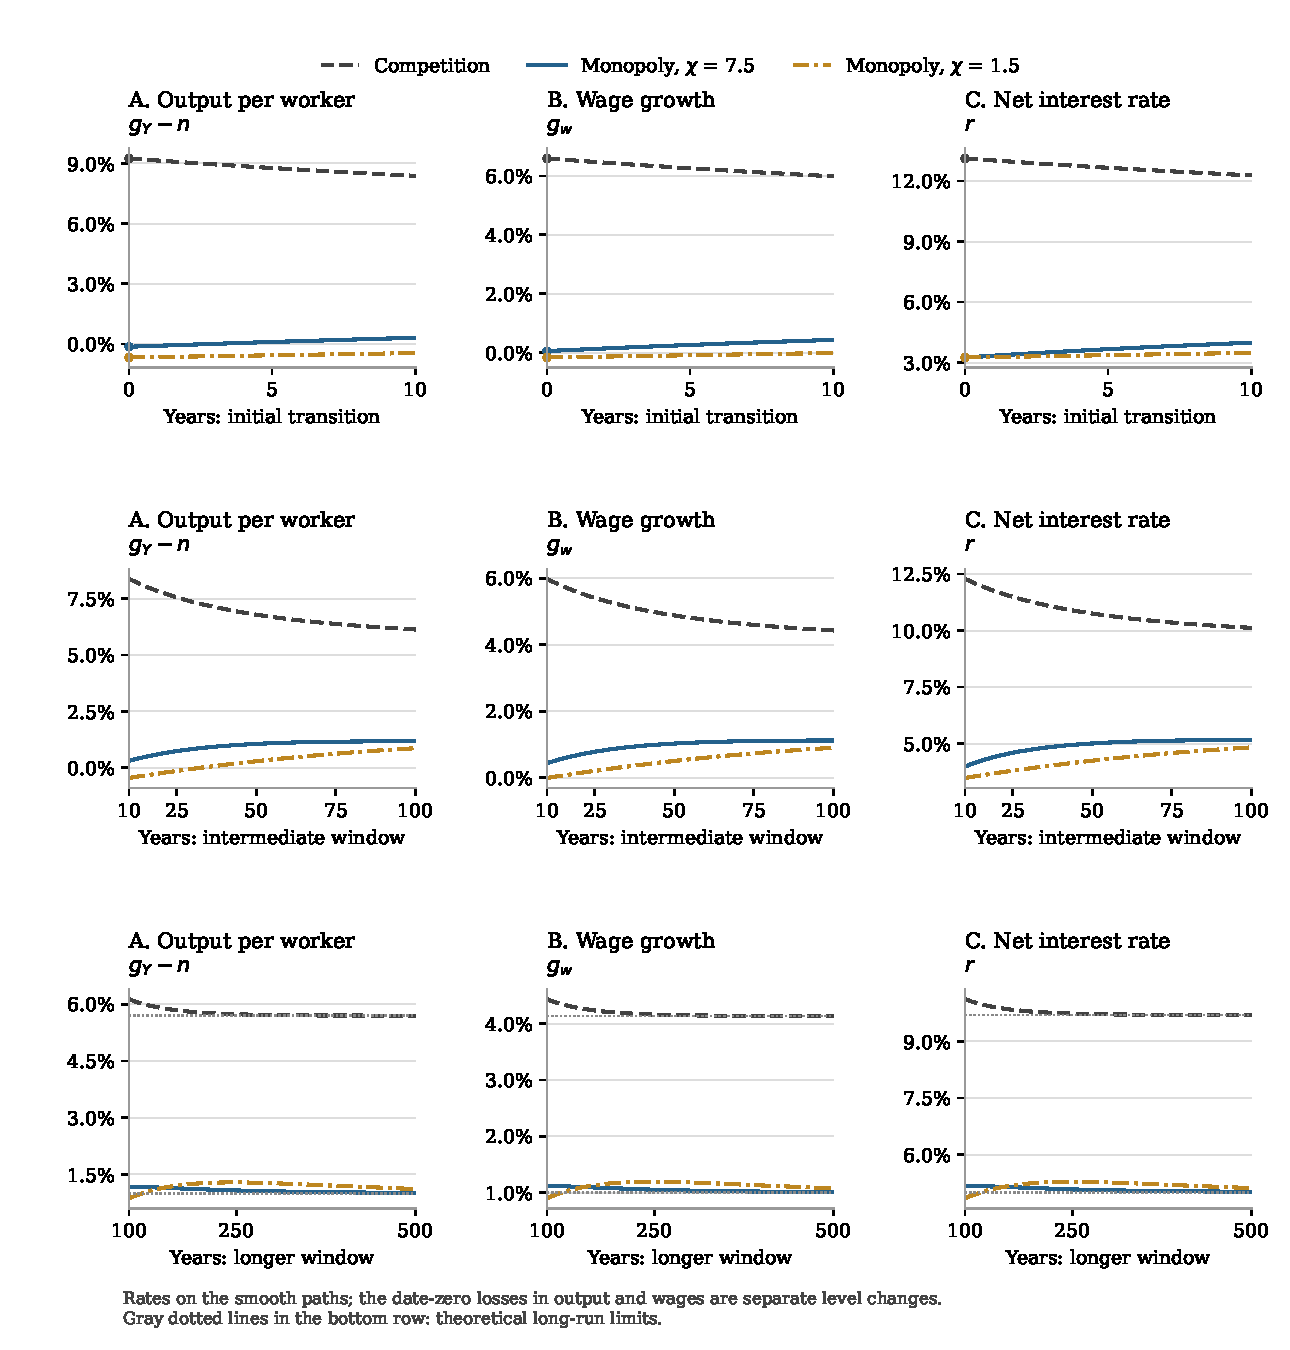
\includegraphics[width=\textwidth]{figures_rewrite/monopoly_growth_reversal/monopoly_growth_reversal_growth.pdf}
 \caption{Monopoly and the loss of AI-dominated growth: annual
 output-per-worker growth, wage growth, and net interest. Rows show
 years 0--10, 10--100, and 100--500. Rates describe the smooth paths
 in each scenario, not the instantaneous output and wage
 losses. Gray dotted lines in the bottom row indicate theoretical
 long-run limits. Vertical scales differ across windows.}
 \label{fig:rewrite-monopoly-growth-reversal-growth}
\end{figure}

The longer windows distinguish recovery from sustained acceleration.
Under continued competition, output-per-worker growth tends to
$5.7\%$, wage growth to $4.1\%$, and the interest rate to $9.7\%$,
as in equation~\eqref{eq:rewrite-competitive-ai-growth}.
Under either monopoly path, the corresponding limits are $1.0\%$,
$1.0\%$, and $5.0\%$, consistent with the labor-bottleneck regime in
Proposition~\ref{prop:rewrite-equilibrium-regimes}. Growth can temporarily
exceed its monopoly limit during the adjustment: with $\chi=1.5$,
output-per-worker growth is still $1.1\%$ at year 500. Monopoly removes
the permanently faster growth, not all growth, and the transition is
not a monotonic decline in growth rates.

Figure~\ref{fig:rewrite-monopoly-growth-reversal-technology} explains
why efficiency gains do not prevent this outcome. Using the same lines
and windows, panels A--C show $B/\overline B$, AI services relative to
continued competition, and labor income as a share of output.
In the first decade, monopoly raises efficiency but supplies fewer
AI services than competition. In the longer run, efficiency approaches
$\overline B$, an improvement of $11.1\%$ over $B_0$; competition
retains $B_0$. Yet the monopoly markup prevents these improvements
from sustaining the joint expansion of capital and AI services that
occurs under competition. AI services under monopoly become negligible
\emph{relative to the competitive path}, not in absolute terms.
Labor's income share tends to $4.5\%$ under monopoly rather than zero
under competition. This larger share coexists with slower wage growth;
at year 500, the low-research-productivity path is still adjusting,
with a labor share of $4.8\%$.

\begin{figure}[tp]
 \centering
 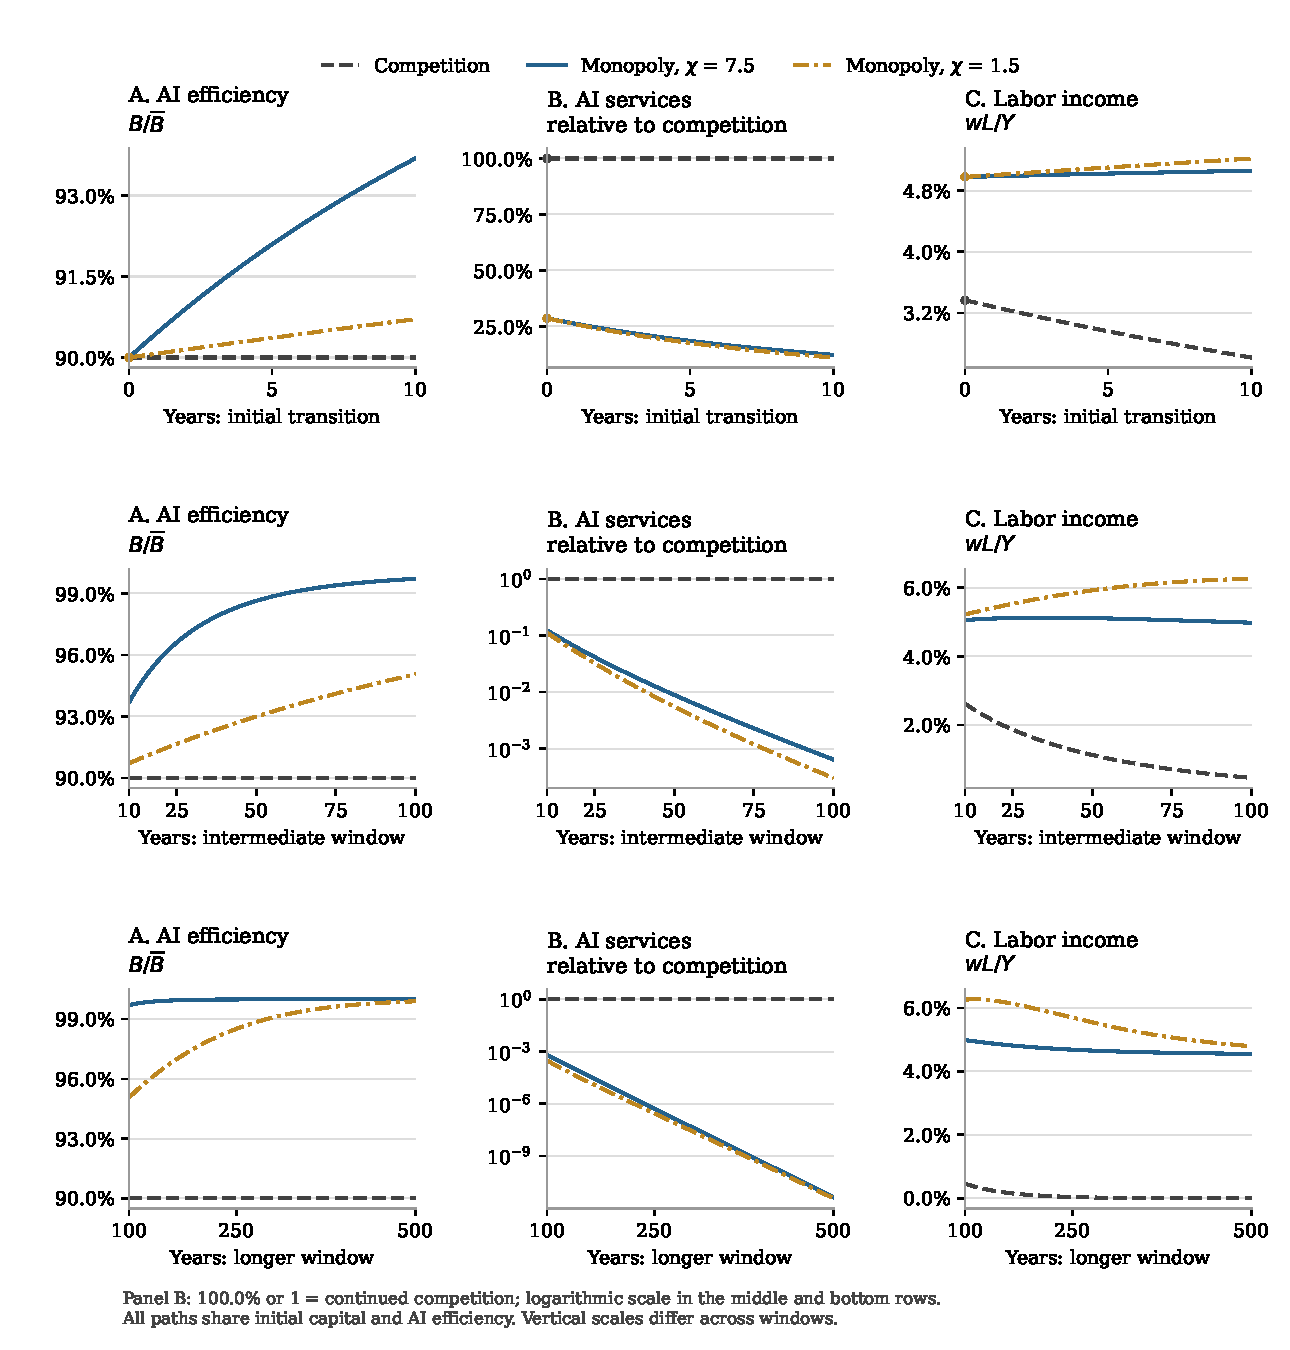
\includegraphics[width=\textwidth]{figures_rewrite/monopoly_growth_reversal/monopoly_growth_reversal_technology.pdf}
 \caption{More efficient AI but slower growth under monopoly:
 efficiency relative to its upper bound, AI services relative to
 continued competition, and labor's income share. Windows and line
 styles match Figure~\ref{fig:rewrite-monopoly-growth-reversal-growth}.
 Panel B uses percentages in the first row and multiples on logarithmic
 scales in the lower rows; its competitive benchmark is $100.0\%$ or
 one. Vertical scales differ across windows.}
 \label{fig:rewrite-monopoly-growth-reversal-technology}
\end{figure}

This experiment deliberately starts with relatively efficient AI and
limited scope for further improvement. Its large initial adjustments
also reflect the abrupt withdrawal of access to existing technology.
I use it to illustrate a possible growth reversal, not to predict the
effects of an actual monopoly grant or rank household welfare.
Appendix~\ref{app:rewrite-competitive-transition} describes the additional
competitive-transition solver and numerical checks. The preceding
simulations remain separate experiments with different initial states
and efficiency bounds.
\clearpage
